\chapter{Introduction}
\label{ch:introduction}

\section{Notation}
\label{sec:notation}
Please follow the typestting standards in mathematics that the International
Standards Organization (ISO) has established. The most important points in it are: 
  

\begin{enumerate}
\item Simple variables are represented by italic letters as $a,\,x,\,A,\,X$.
\item Vectors are written in boldface italic (uncapitalized) as $\boldsymbol{a,\, x}$.
\item Matrices may appear as boldface italic capital letters as in $\boldsymbol{A,\, X}$
\item Sets are represented by capital script letters as $\mathcal{A}$, $\mathcal{X}$.
\item The special numbers $\mathrm{e}$, $\mathrm{i}$ and the differential operator $\mathrm{d}$ are written in upright roman.
\end{enumerate}
%
%
%
\section{Compilation with latex}
Generally, a \LaTeX\ document is compiled with the command \verb'latex thesis'.
If you use bibtex for your references the typical compilation workflow is: 
\begin{itemize}
	\item \verb'latex thesis'
	\item \verb'bibtex thesis'
	\item \verb'latex thesis'
	\item \verb'latex thesis'
	\item \verb'dvipdf thesis'
\end{itemize}
All graphics must be in the eps format (the eps format is further commented in Section \ref{sec:figures}).

\section{Compilation with pdflatex}
The use of \verb'pdflatex' instead of \verb'latex' has the following benefits:
Pictures can be included as pdf, jpg, and png files 
and the output is directly in pdf (no dvips). The compilation is also faster. 

If you use bibtex the compilation steps should be: 
\begin{itemize}
	\item \verb'pdflatex thesis'
	\item \verb'bibtex thesis'
	\item \verb'pdflatex thesis'
	\item \verb'pdflatex thesis'
\end{itemize}
%
%
%
\section{Figures}
\label{sec:figures}                                     
Figures are handled in the standard \LaTeX\ manner. For example: \\
\verb'\begin{figure}'\\
\verb'  \centering'\\
\verb'  \includegraphics[width=0.8\linewidth]{myfigure}'\\
\verb'  \caption{Simulation Results}'\\
\verb'  \label{fig:label}'\\
\verb'\end{figure}'\\
If you want subfigures, include the subfigure package \verb'\include{subfigure}'.

Make sure that you save your graphics in vector form, which will not degrade or pixelize your graphic when magnified. If you compile with \verb'latex' this would be \verb'myfigure.eps' and for \verb'pdflatex' users \verb'myfigure.pdf'. Both eps and pdf support vector graphics. 

How to generate graphics? Draw all your drawings with a drawing/graphic application that supports vector graphics. 
My favourite is OpenOffice Draw. Alternatives include Adobe Illustrator, sK1, Inkscape, Xara Xtreme. 
These application save your drawing automatically in vector form; if you include a photo it is usually still saved in bitmap form.
Matlab plots can be directly saved as eps/pdf. Note that Matlab saves pdfs in DINA4 size. You can crop the pdf with the shell command \verb'pdfcrop myfigure.pdf'. 

The psfrag package might be of interest for \verb'latex' users. Psfrag allows the user to "go into" an eps graphic and replace text
strings contained in it with real \LaTeX\ code (works not with pdflatex). 

\begin{figure}[htb]
	\centering
	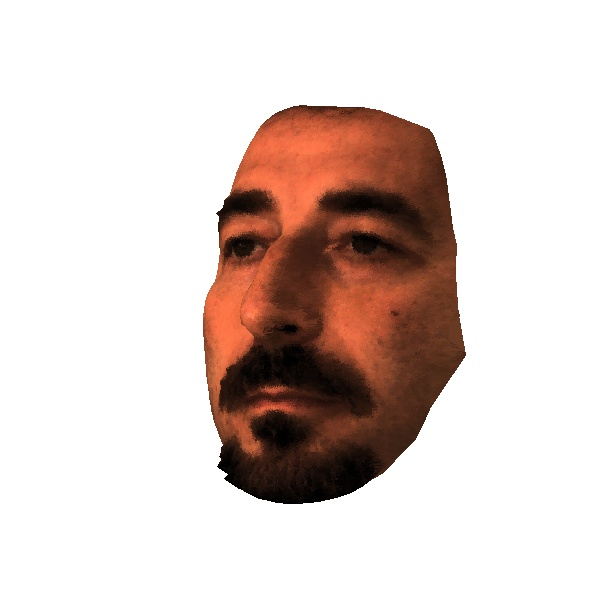
\includegraphics[width=0.35\linewidth]{figures/figure}
	\caption{Some sample figure.}
	\label{fig:sample}
\end{figure}

\begin{figure}[htb]
	\centering
	\subfigure[Matlab plot exported directly as eps/pdf which saves the plot in vector form. Note the nice quality even though it has been rescaled.]{
		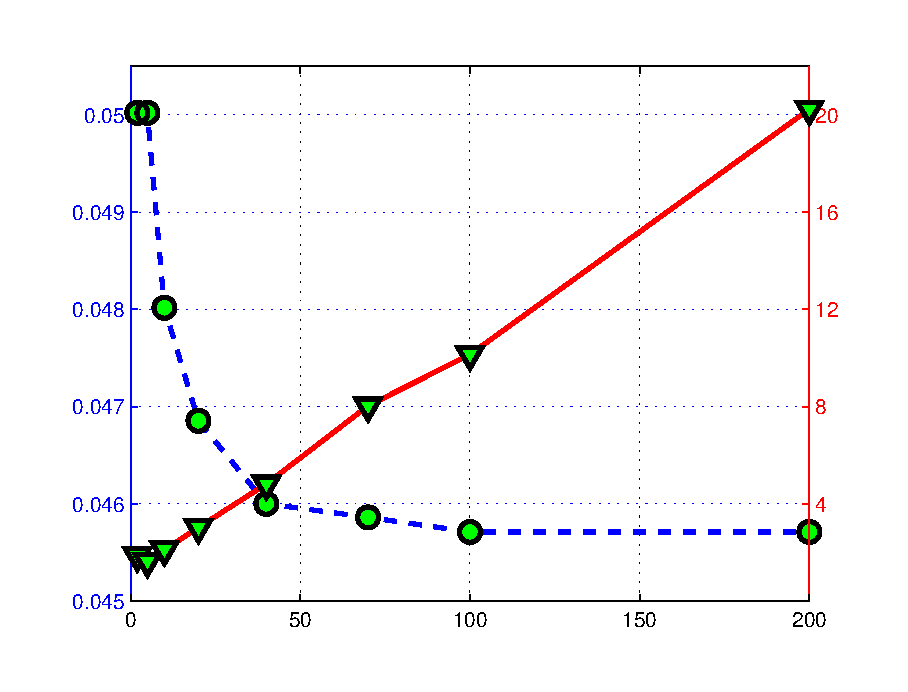
\includegraphics[width=0.85\linewidth]{figures/varyM}
		\label{fig:matlabgood}
	}
	\subfigure[Matlab plot saved in bitmap form. The quality is bad. Remember: Export your figures as vector graphic if possible.]{
		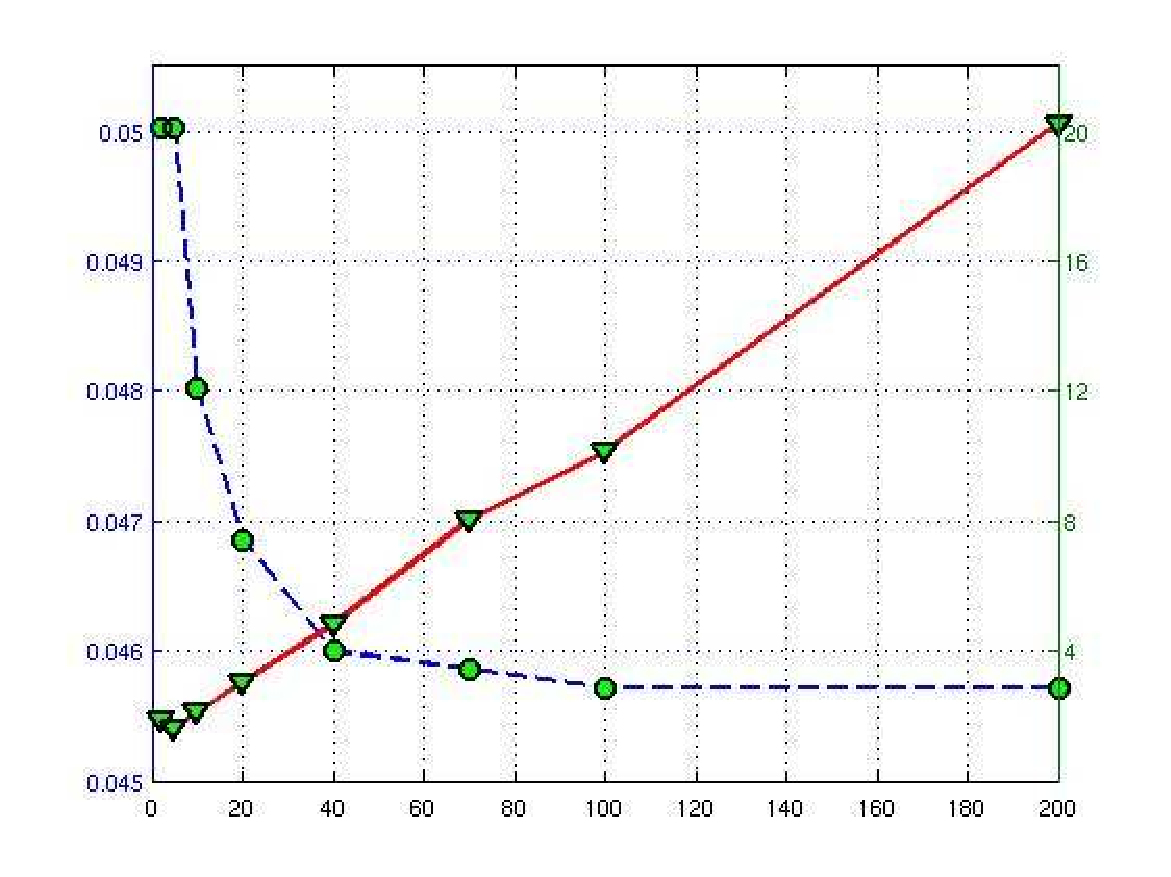
\includegraphics[width=0.85\linewidth]{figures/varyM_jpg}
		\label{fig:matlabbad}
	}
\end{figure}

\section{Clean Bibliography}
Go to \verb'http://dblp.mpi-inf.mpg.de/dblp-mirror/index.php' and search for the paper you want to cite. 
You can copy the bibtex entry from there directly to your bibliography file, so that all the references have the same look. 
%
%
%
\section{\LaTeX\ Literature}
My favourite \LaTeX\ tutorial is the \LaTeX\ primer written by Krishnan \cite{Kr03} and a quite comprehensive book is \cite{Ko03}, of which the library has adequate stock.  


